\question{Токи в диодном промежутке при наличии переменного напряжения между
  электродами}

Анализ движения электронов в диодном промежутке при наличии пространственного 
заряда показывает, что величина анодного тока определяется законом Ленгмюра
\begin{equation}
	I_a = PU_a^{3/2}
	\label{eq24.1.1}
\end{equation}
где 
\[
	P = \frac{4}{9}\eps_0
		\sqrt{2\left| \frac{e}{m} \right|}\frac{S_k}{d^2} 
\] 
первеанс диода; \( S_k \) -- площадь катода, \( d \) -- расстояние 
катод-анод.

Результаты эксперимента достаточно хорошо согласуются с соотношением 
(\ref{eq24.1.1}) не только в статическом режиме, но и при подаче переменного 
напряжения между электродами до тех пор, пока время пролёта электрона от 
катода до анода, определяемое по классическим законам динамики Ньютона 
\[
	t_a = d\sqrt{\frac{2}{U_{a0}}\left| \frac{m}{e} \right|}
\]
не становится сравнимым с периодом высокочастотных колебаний
\[
	T = \frac{2\pi}{\omega}
\]

Затем характер зависимости величины тока от прикладываемого напряжения 
начинает существенно изменяться. 

Рассмотрим физическую природу тока в данном промежутке при наличии 
высокочастотных полей. Для упрощения анализа предположим, что анод и катод 
представляют собой две параллельные плоскости, расположенные на расстоянии 
\( d \) друг от друга. Считаем, что катод представляет собой частую сетку, 
абсолютно прозрачную для электронов. От катода к аноду движется тонкий слой 
электронов со скоростью \( v \). Анод и катод замкнуты накоротко вне диода, 
что устраняет внешнее, не обусловленное движение электронов, электрическое 
поле (рис.\ref{img24.1}).

\begin{figure}[h!]
	\center
	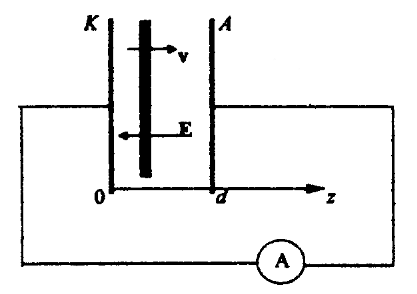
\includegraphics[width=.4\textwidth]{24_1}
	\caption{Диодный промежуток}
	\label{img24.1}
\end{figure}

В этом случае слой зарядов будет двигаться в диодном промежутке только за 
счёт энергии, сообщенной ему вне этого пространства каким-либо внешним 
устройством.

При введенных предположениях все процессы зависят только от координаты, и 
полная плотность тока определяется как сумма плотностей тока проводимости 
\[
	j_\text{пр} = \sigma E
\]
конвекционного тока
\begin{equation}
	j_k = -\rho v
	\label{eq24.1.5}
\end{equation}
и тока смещения 
\begin{equation}
	j_\text{см} = \eps_0 \pder{E}{t}
	\label{eq24.1.6}
\end{equation}
\begin{equation}
	j = j_\text{пр} + j_k + j_\text{см}
	\label{eq24.1.7}
\end{equation}

В (\ref{eq24.1.5}) и далее учтено, что рассматривается движение электронов, 
поэтому взят знак минус перед зарядов в (\ref{eq24.1.5}).

Поскольку в диодном промежутке \( \sigma = 0 \), то 
\begin{equation}
	j = j_k + j_\text{см}
	\label{eq24.1.8}
\end{equation}

Кроме этого, из уравнения Максвелла \( \div\vec{E} = -\rho/\eps_0 \) в 
предположении зависимостей всех функций только от \( z \) и \( t \) следует, 
что 
\begin{equation}
	\rho = -\eps_0 \pder{\vec{E}}{z}
	\label{eq24.1.9}
\end{equation}

Из (\ref{eq24.1.5}), (\ref{eq24.1.6}), (\ref{eq24.1.8}) и (\ref{eq24.1.9}) следует 
\[
	j = -\left( 
		\eps_0\pder{\vec{E}}{t} + \eps_0\pder{\vec{E}}{z}\frac{dz}{dt}
	\right) = -\eps_0 \frac{d\vec{E}}{dt}
\]

Иначе, плотность полного тока представляет собой полную производную 
напряженности электрического поля по времени.

Ввиду непрерывности и замкнутости линий полного тока можно утверждать, что 
через любое сечение диода при \( z = const \) проходит один и тот же полный 
ток. Но это утверждение не относится отдельно к конвекционному току или току 
смещения. 

Рассмотрим следующий пример. Пусть плоский слой электронов толщиной 
\( 2\Delta \ll d \), на единицу площади которого приходится заряд \( \sigma \) 
влетает в диодный промежуток.

\begin{figure}[h!]
	\center
	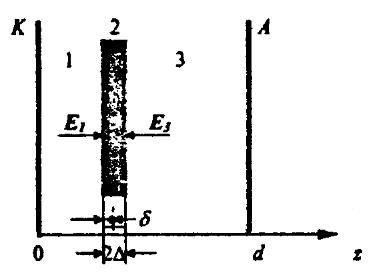
\includegraphics[width=.4\textwidth]{24_2}
	\caption{Распределение полей, обусловленных действием пространственного 
		заряда, в диодном промежутке}
	\label{img24.2}
\end{figure}

Тогда объёмная плотность \( \rho = \sigma / 2\Delta \), а плотность 
конвекционного тока 
\begin{equation}
	j = -\frac{\sigma}{2\Delta}v = \frac{|\sigma|}{2\Delta} v
	\label{eq24.1.11}
\end{equation}

С учётом того, что \( |\sigma| = -\sigma \) (поток электронов).

Если считать, что слой тонкий, то, согласно граничным условиям нормальная 
составляющая электрического поля терпит разрыв, равный 
\begin{equation}
	E_1 - E_3 = \frac{\sigma}{\eps_0} = -\frac{|\sigma|}{\eps_0}
	\label{eq24.1.12}
\end{equation}

Поскольку векторы \( \vec{E}_1 \) и \( \vec{E}_3 \) коллинеарны, в 
(\ref{eq24.1.12}) учтены только их абсолютные значения.

С другой стороны, поскольку между катодом и анодом не подано внешнее 
напряжение (рис.\ref{img24.1}, то общее напряжение в промежутке равно нулю, 
то есть
\begin{equation}
	E_1 z + E_3 (d-z) = 0
	\label{eq24.1.13}
\end{equation}

Из (\ref{eq24.1.5}) и (\ref{eq24.1.8}) следует, что
\[
	\left. \begin{array}{c}
		E_1 = -\frac{|\sigma|}{\eps_0}\frac{d-z}{d}; \\
		E_3 = \frac{|\sigma|}{\eps_0}\frac{z}{d}.
	\end{array} \right\}
\]

Иначе, над потоком поле имеет направление, при котором лоренцева сила 
направлена к аноду, а под потоком -- к катоду.

Внутри слоя напряженность изменяется линейно за счёт сил пространственного 
заряда
\[
	E_2 = E_1 + \frac{|\sigma|}{\eps_0}\frac{\delta}{2\Delta}
\]

(\( \delta \) -- расстояние от рассматриваемой точки \( a \) до левой границы 
электронного слоя), в связи с чем удовлетворяются условия при \( \delta = 0 \) 
(\( E_1 = E_2 \)) и при \( \delta = 2\Delta \) (\(E_2 = E_3 \)).

При движении слоя появляются токи смещения в каждой из областей:
\begin{equation}
	\left. \begin{array}{c}
		j_\text{см1} = \eps_0 \pder{E_1}{z} = 
			\frac{|\sigma|}{d}\frac{dz}{dt} = \frac{|\sigma|}{d} v; \\
		j_\text{см3} = \eps_0 \pder{E_3}{z} = 
			\frac{|\sigma|}{d}\frac{dz}{dt} = \frac{|\sigma|}{d} v; \\
		j_\text{см2} = \eps_0 \pder{E_2}{z} = 
			\frac{|\sigma|}{d}\frac{dz}{dt} = \frac{|\sigma|}{d} v + 
			\frac{|\sigma|}{2\Delta}\frac{d\delta}{dt}.	
	\end{array} \right\}
	\label{eq24.1.16}
\end{equation}

Поскольку положение рассматриваемой точки фиксировано, то при движении 
слоя скорость уменьшения \( \delta(t) \) пропорциональна скорости движения 
левой границы слоя, то есть
\[
	\frac{d\delta(t)}{dt} = -v
\]
В результате из (\ref{eq24.1.16}) находим 
\[
	j_\text{см2} = \frac{|\sigma|}{d} v + \frac{|\sigma|}{2\Delta}v
\]
а плотность полного тока, равная сумме плотностей тока смещения и 
конвекционного тока (\ref{eq24.1.11}), равна
\[
	j = \frac{|\sigma|}{d}v
\]

Таким образом, в области 2 величина плотности полного тока совпадает с 
величинами наведенных токов в областях 1 и 3. При этом полный ток не зависит 
от величины объёмной плотности пространственного заряда, а определяется 
полным в слое, так как 
\begin{equation}
	i_\text{полн} = j_\text{полн}S = \frac{|q|}{d}v
	\label{eq24.1.18}
\end{equation}
(\(S\) -- площадь поперечного сечения слоя). При этом величина наведенного 
тока в областях 1 и 3 равна величине полного тока в области потока. 

Если диодный промежуток заполнен непрерывно движущимися зарядами, то 
наведенный ток определяется как интеграл по всем электронным слоям:
\[
	i_\text{нав} = \frac{1}{d}\int\limits_V |dq| v
\]

Поскольку в этом случае заряд \( |dq| \) расположен внутри некоторого объёма 
\( dV \), то, вводя величину объёмной плотность заряда 
\( |\rho| = |dq|/dV \), и учитывая, что \( j_k = -\rho v = |\rho|v \), 
получаем 
\begin{equation}
	i_\text{нав} = \frac{1}{d}\int\limits_V j_k dV = 
		\frac{1}{d} \int\limits_V |\rho| dV
	\label{eq24.1.19}
\end{equation}

В соотношении (\ref{eq24.1.19}) учтено, что на электрод не подаётся внешнее 
напряжение. Если же между электродами прикладывается некоторое напряжение 
\( U \), то полный ток складывается из тока, обусловленного движением 
электронов, и тока, создаваемого за счёт внешнего электрического поля. 

Первая часть -- это индуцированные токи, вызванные движением зарядов. 

Вторая часть -- это токи смещения, создаваемые приложенным напряжением. 
Наличие электронов не влияет на его величину, так как 
\[
	j_\text{см.вн} = \eps_0 \pder{E_\text{вн}}{t}
\]
а распределение определяется только геометрией электродов и частотой внешнего 
сигнала.

При отсутствии электронов в пространстве катод-анод величина напряженности 
электрического поля
\[
	E_u = \frac{U_0}{d}
\]
Если теперь рассмотреть тонкий плоский слой электронов на расстоянии 
\( z \ll d \) от катода (рис.\ref{img24.2}), величина поверхностной плотности 
которого \( \sigma = -|\sigma| \), из условия разрыва нормальных составляющих 
напряженности электрического поля получаем как и в (\ref{eq24.1.12})
\[
	E_1 - E_3 = \frac{\sigma}{\eps_0} = -\frac{|\sigma|}{\eps_0}
\]
но для потенциала соотношение будет иное:
\[
	E_1 z + E_3(d-z) = U_0 = E_u d
\]
и из (\ref{eq24.1.12}) и предыдущего выражения находим:
\[
	\begin{array}{c}
		E_1 = E_u - \frac{|\sigma|}{\eps_0}\left( 1 - \frac{z}{d}\right); \\
		E_3 = E_u + \frac{|\sigma|}{\eps_0}\frac{z}{d}
	\end{array}
\]

Таким образом, над потоком величина напряженности поля больше, чем под ним.

В общем случае при наличии пространственного заряда во всём диодном промежутке 
напряженность поля может быть определена из условия суммирования напряженности 
внешнего поля \( E_u \) и поля, обусловленного пространственного зарядом, 
распределенном во всём объёме:
\[
	\oint\limits_S \vec{E}_\text{пз} \vec{n} dS = 
		\frac{1}{\eps_0}\int\limits_V \rho dV = 
		\frac{1}{\eps_0}\int\limits_S dS \int\rho dz
\]
откуда, учитывая одномерный характер движения, получаем 
\[
	E_\text{пз} = -\frac{1}{\eps_0}\int|\rho|dz
\]
В результате
\[
	E(z,t) = E_u - \frac{1}{\eps_0}\int|\rho|dz
\]